\chapter{Notificaciones}
\label{mod:13-notificaciones}

\section{Propósito}
\label{sec:notificaciones-proposito}

Centro de alertas internas para el staff de la óptica: avisa de eventos que requieren atención (stock bajo, una transferencia de stock pendiente de aceptar, un pedido de laboratorio recibido) sin que nadie tenga que revisar manualmente cada pantalla. El diseño de destinatario (usuario, sucursal o global) es la base sobre la que se apoyan las preferencias de notificación configurables por cada persona.

\section{Entidades principales}
\label{sec:notificaciones-entidades}

\begin{longtable}{p{3.6cm}p{9.6cm}}
\caption{Entidad principal del módulo de Notificaciones.}\label{tab:notificaciones-entidades}\\
\toprule
\textbf{Entidad} & \textbf{Rol} \\
\midrule
\endfirsthead
\toprule
\textbf{Entidad} & \textbf{Rol} \\
\midrule
\endhead
\bottomrule
\endfoot
\code{Notificacion}\allowbreak \code{Interna} & Una alerta: destinatario (usuario / sucursal / global), tipo, mensaje, leída o no \\
\end{longtable}

Ver Capítulo~\ref{sec:modelo-datos} (entidad transversal, no pertenece a ninguno de los 3 grupos del DER --- se referencia desde ahí).

\section{Reglas de negocio clave}
\label{sec:notificaciones-reglas}

\begin{itemize}
  \item \textbf{Scoping de destinatario en 3 niveles}, resuelto vía \code{ICurrent}\allowbreak \code{User}\allowbreak \code{Context}: \code{Destinatario}\allowbreak \code{Usuario}\allowbreak \code{Id} (individual), \code{Destinatario}\allowbreak \code{Sucursal}\allowbreak \code{Id} (broadcast a todo el staff de esa sucursal), o ambos \code{null} (broadcast global). No existe scoping por rol --- los roles son dinámicos y \code{ICurrent}\allowbreak \code{User}\allowbreak \code{Context} no expone el nombre de rol de forma robusta.
  \item \textbf{\code{Leido} es un único flag compartido} en las notificaciones de broadcast, no por-usuario --- decisión explícita: si dos personas del staff comparten una notificación de sucursal, cuando una la marca como leída desaparece para ambas. Ver \hyperref[adr:0010]{ADR 0010 --- Notificaciones internas antes que externas}.
  \item \textbf{La visibilidad de broadcasts exige el permiso concreto \code{ver_}\allowbreak \code{todas_}\allowbreak \code{sucursales}}, no se infiere de \code{ICurrentUserContext.}\allowbreak \code{EsGlobal} (que también es \code{true} para pacientes, ver \hyperref[adr:0009]{ADR 0009}) --- así un paciente con \code{ver_}\allowbreak \code{notificaciones} nunca ve los broadcasts operativos de otras sucursales.
  \item \textbf{Tres triggers reales conectados} (no hooks genéricos, cada uno cableado a mano):
  \begin{enumerate}
    \item \textbf{Bajo stock} --- \code{Stock}\allowbreak \code{Bajo}\allowbreak \code{Notificador}\allowbreak \code{Service}, un \code{BackgroundService} que hace polling cada 30 minutos (mismo patrón que \code{Turno}\allowbreak \code{Reminder}\allowbreak \code{Service}) comparando \code{vw_stock_actual} contra \code{Producto}\allowbreak \code{Stock}\allowbreak \code{Config} por Producto más Sucursal. Se eligió poller en vez de hook inline porque los movimientos de stock ``Aprobado'' se originan desde al menos 5 servicios distintos (Compras, Ventas, Recepciones, Conteos, Transferencias) --- instrumentar los 5 hubiera sido más invasivo que un poller. No duplica si ya hay una notificación sin leer para el mismo producto más sucursal.
    \item \textbf{Transferencia pendiente} --- hook directo en \code{TransferenciaStockService.}\allowbreak \code{CreateAsync}.
    \item \textbf{Pedido de laboratorio recibido} --- hook directo en \code{LaboratorioService.}\allowbreak \code{RegistrarRecepcionAsync}.
  \end{enumerate}
\end{itemize}

\section{Endpoints}
\label{sec:notificaciones-endpoints}

\begin{longtable}{p{2cm}p{6cm}p{5.9cm}}
\caption{Endpoints del módulo de Notificaciones.}\label{tab:notificaciones-endpoints}\\
\toprule
\textbf{Método} & \textbf{Ruta} & \textbf{Descripción} \\
\midrule
\endfirsthead
\toprule
\textbf{Método} & \textbf{Ruta} & \textbf{Descripción} \\
\midrule
\endhead
\bottomrule
\endfoot
GET & \texttt{/api/notificaciones?solo}\allowbreak \texttt{NoLeidas\&page\&pageSize} & Notificaciones del usuario autenticado \\
GET & \code{/}\allowbreak \code{api/}\allowbreak \code{notificaciones/}\allowbreak \code{contador} & Cantidad de no leídas (badge del header) \\
PUT & \code{/}\allowbreak \code{api/}\allowbreak \code{notificaciones/}\allowbreak \code{{id}/leer} & Marca una como leída \\
PUT & \code{/}\allowbreak \code{api/}\allowbreak \code{notificaciones/}\allowbreak \code{leer-todas} & Marca todas como leídas \\
\end{longtable}

Todos bajo policy \code{ver_}\allowbreak \code{notificaciones}. Ver Apéndice~\ref{sec:api-reference}, \S\ref{sec:api-notificaciones}.

\section{Flujo típico}
\label{sec:notificaciones-flujo}

El trigger de bajo stock (poller en background) y el consumo desde el frontend son dos flujos independientes; se muestran por separado.

\begin{figure}[htbp]
\centering
\begin{tikzpicture}
  \node[actor, minimum width=3.6cm] (poller) at (0,0) {StockBajoNotificadorService};
  \node[actor, minimum width=3.6cm] (db) at (5.2,0) {vw\_stock\_actual /\\ ProductoStockConfig};
  \node[actor, minimum width=3.6cm] (n) at (10.4,0) {NotificacionInterna};

  \draw[lineavida] (poller.south) -- ++(0,-4.2);
  \draw[lineavida] (db.south) -- ++(0,-4.2);
  \draw[lineavida] (n.south) -- ++(0,-4.2);

  \draw[mensaje] ($(poller.south)+(0,-1)$) -- node[above,font=\scriptsize]{comparar stock vs. mínimo (cada 30 min)} ($(db.south)+(0,-1)$);
  \draw[mensajeretorno] ($(db.south)+(0,-1.8)$) -- node[below,font=\scriptsize]{stock bajo, sin notificación previa sin leer} ($(poller.south)+(0,-1.8)$);
  \draw[mensaje] ($(poller.south)+(0,-2.8)$) -- node[above,font=\scriptsize]{crear (DestinatarioSucursalId)} ($(n.south)+(0,-2.8)$);
\end{tikzpicture}
\caption{Trigger de bajo stock: polling cada 30 minutos, sin duplicar avisos ya generados y sin leer.}
\label{fig:seq-notificaciones-poller}
\end{figure}

\begin{figure}[htbp]
\centering
\begin{tikzpicture}
  \node[actor, minimum width=3.4cm] (fe) at (0,0) {AppHeader (bell icon)};
  \node[actor, minimum width=3.4cm] (n) at (6,0) {NotificacionInterna};

  \draw[lineavida] (fe.south) -- ++(0,-5);
  \draw[lineavida] (n.south) -- ++(0,-5);

  \draw[mensaje] ($(fe.south)+(0,-1)$) -- node[above,font=\scriptsize]{GET /contador (polling del front)} ($(n.south)+(0,-1)$);
  \draw[mensajeretorno] ($(n.south)+(0,-1.8)$) -- node[below,font=\scriptsize]{cantidad no leídas $\to$ badge} ($(fe.south)+(0,-1.8)$);
  \draw[mensaje] ($(fe.south)+(0,-2.8)$) -- node[above,font=\scriptsize]{GET /notificaciones (dropdown, últimas 5)} ($(n.south)+(0,-2.8)$);
  \draw[mensaje] ($(fe.south)+(0,-4)$) -- node[above,font=\scriptsize]{PUT /{id}/leer} ($(n.south)+(0,-4)$);
\end{tikzpicture}
\caption{Consumo desde el frontend: badge de contador, listado desplegable y marcado de lectura.}
\label{fig:seq-notificaciones-frontend}
\end{figure}

Los otros dos triggers (transferencia pendiente, laboratorio recibido) son hooks síncronos dentro del flujo de negocio correspondiente, sin polling --- se disparan en el mismo request que crea la transferencia o registra la recepción.

\section{Vistas de frontend}
\label{sec:notificaciones-frontend}

\begin{itemize}
  \item \code{NotificacionesView.}\allowbreak \code{vue} --- listado completo (reemplazó un placeholder \code{ComingSoonView} en \code{/notificaciones})
  \item Bell icon más dropdown en \code{AppHeader.vue} (componente global, no vista): badge de contador, últimas 5, marcar leída, link ``Ver todas''
\end{itemize}

\section{Interfaz}
\label{sec:notificaciones-interfaz}

\begin{figure}[htbp]
\centering
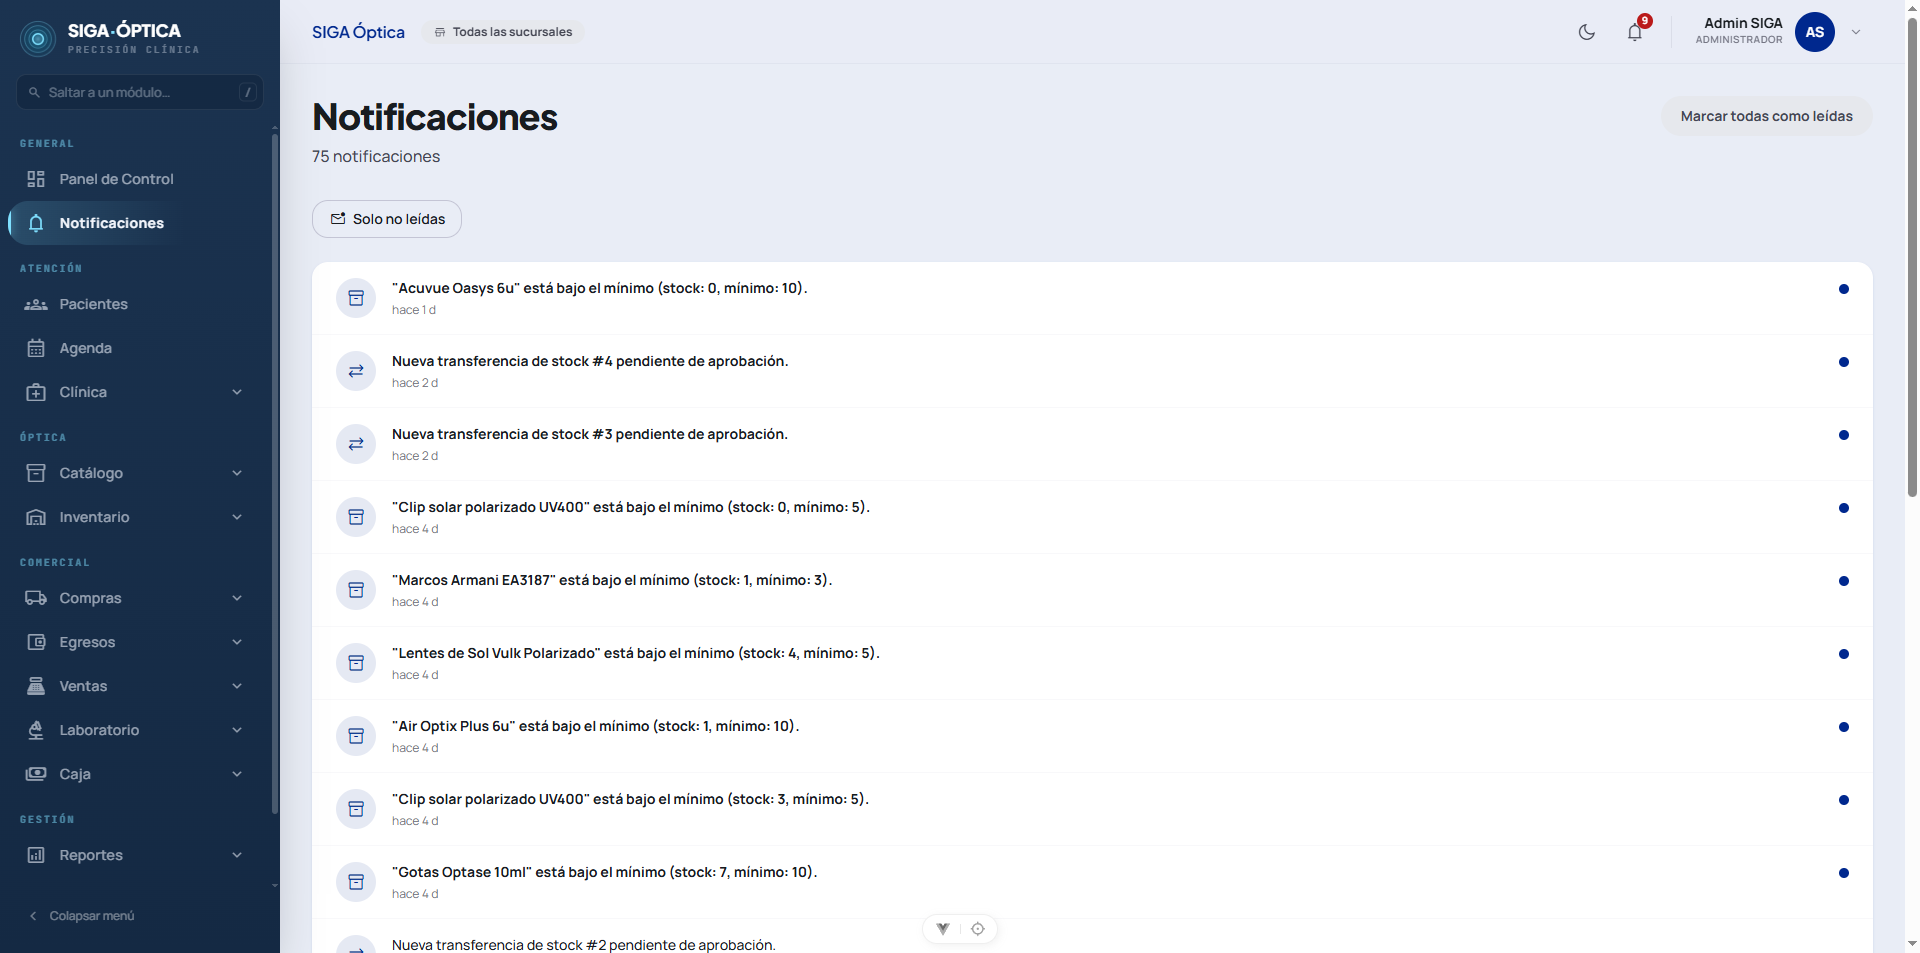
\includegraphics[width=0.95\textwidth]{imagenes/mod13-notificaciones.png}
\caption{Centro de notificaciones internas, con avisos de stock bajo y transferencias pendientes de aprobación.}
\label{fig:mod13-notificaciones}
\end{figure}

\section{Estado}
\label{sec:notificaciones-estado}

\Implementado\ Fase 1 (centro interno): migración \code{055_}\allowbreak \code{NotificacionesInternas}, poller de bajo stock generando notificaciones reales, y los 4 endpoints del centro de notificaciones.
